\subsection{従来のmemo,latex,hiki}
\begin{figure}[htbp]\begin{center}
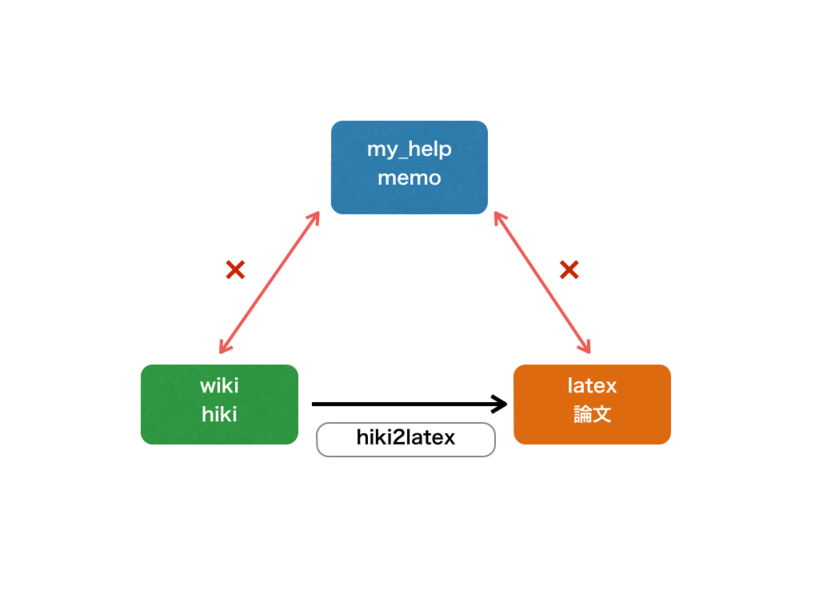
\includegraphics[width=10cm,bb= 0 0 737 453]{../figs/./my_help2hiki_saki.003.png}
\caption{ memo,latex,hikiの比較}
\label{default}\end{center}\end{figure}
\subsubsection{my\_help}
my\_helpは,メモを作るためのgem.
ユーザがターミナルを利用して作成し,閲覧する.
メモの書式はyaml形式で,拡張子は.ymlを使用している.

\subsubsection{wiki}
miというmacのテキストエディタを用いて作成する.
作成したファイルはMac OSのブラウザのsafariで開くことができる.
hiki形式で記述し,webを通して誰でも見られるようにできる.

\subsubsection{latex}
TeXの書式で,TeX編集用エディタのTeXShopによって作成する.
pdfは一般的に使われている電子ファイルで,印刷して卒業論文の
ハードコピーとしても使われる.

このようにmy\_help,wiki,latexは書式や作成,閲覧方法が全て違う.
目的も異なるので,同じ内容のファイルをそれぞれの書式で書かなければならないことがある.

\begin{figure}[htbp]\begin{center}
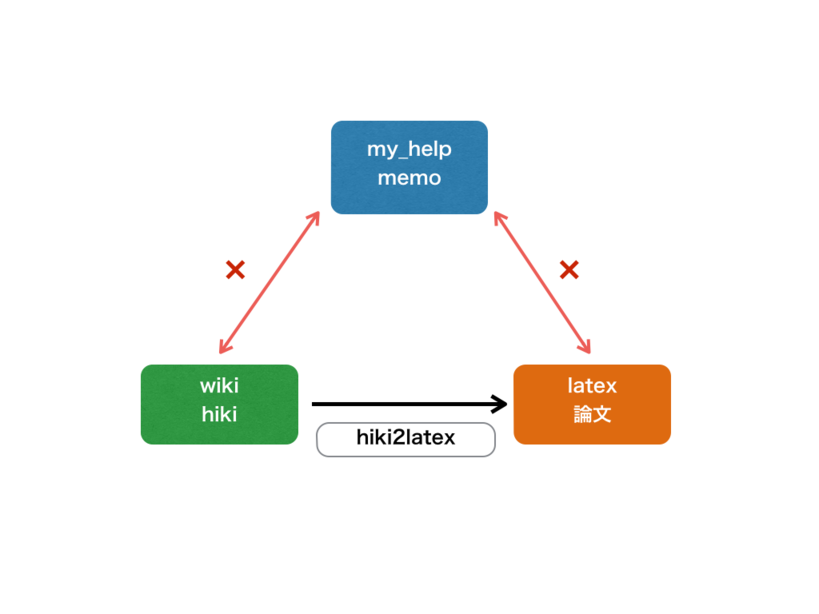
\includegraphics[width=10cm,bb= 0 0 737 453]{../figs/./my_help2hiki_saki.004.png}
\caption{ hiki2latex}
\label{default}\end{center}\end{figure}
hiki2latexの開発により上図のようにwikiとlatexの変換はできるようになったが,
my\_helpとwiki,my\_helpとlatexは関連させることができなかった.
本研究により,my\_help,wiki,latexを関連させるため,
my\_helpからwikiへ自動変換を行うシステムmy\_help2hikiの開発を目指す.

\begin{figure}[htbp]\begin{center}
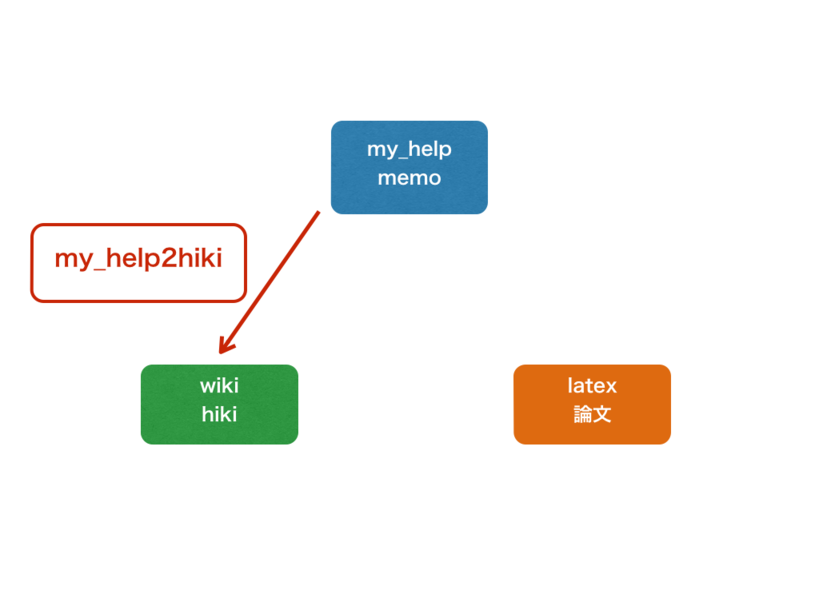
\includegraphics[width=10cm,bb= 0 0 737 453]{../figs/./my_help2hiki_saki.005.png}
\caption{my\_help2hiki}
\label{default}\end{center}\end{figure}
